\documentclass[border = .2cm]{standalone}
 
\usepackage{pgfplots}

\pgfplotsset{compat = newest}
\definecolor{mblue}{RGB}{31,119,180}

\pgfplotsset{
    colormap={cmblue}{
            rgb255(0cm)=(132,233,233);
            rgb255(1cm)=(66,164,233);
            rgb255(2cm)=(132,233,233);
        },
    colormap={whiteblack}{color=(black) color=(white)},
    tick label style={color=white},
}

\begin{document}
 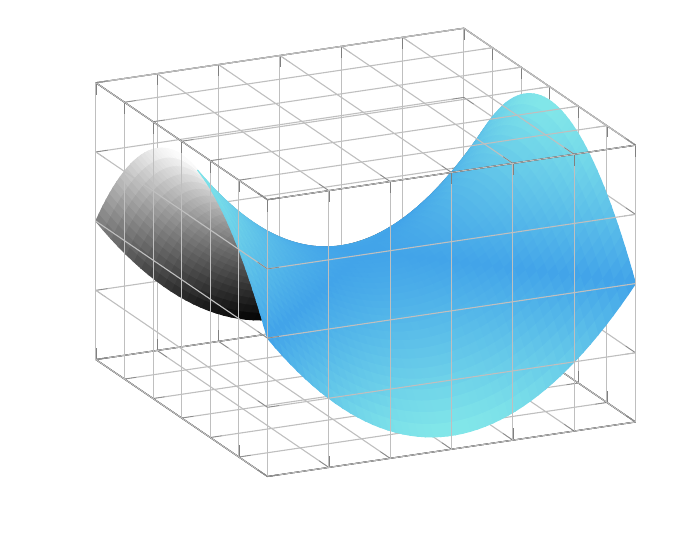
\begin{tikzpicture}
 
    \begin{axis}[
        view = {-25}{25},
        mesh/interior colormap name=cmblue, colormap name=whiteblack,
        xmax = +3,
        xmin = -3,
        ymax = +3, 
        ymin = -3, 
        zmax = +10, 
        zmin = -10,
        xtick = {-3,-2,-1,0,1,2,3},
        ytick = {-3,-2,-1,0,1,2,3},
        ztick = {-10,-5,0,5,10},
        grid,
        3d box = complete*
        ]
        
    \addplot3 [
        domain = -3:3,
        domain y = -3:3,
        samples = 50,
        samples y = 50,
        surf,
        shader = flat
        ] {x^2 - y^2};
 
\end{axis}
 
\end{tikzpicture}
\end{document}
